\section{Experiment Design}
\label{sec:experimentdesign}

To study band selection in multiple area types, we developed static and driving experiments 
on off-the-shelf wireless platform and remote controlled spectrum analyzer platform.
According to the measured data, we apply our access point deploymnet framework to analyze
 white space band performance in typical downtown, urban, rural and intercetion areas.


% Platform
To ensure the results are applicable, we employ a Linux-based 802.11 testbed~\cite{Gateworks}.
The platform includes a Gateworks 2358 node with Ubiquiti XR radios (XR9 at 900 MHz, 
XR2 at 2.4 GHz, XR5 at 5.2 GHz) and a DoodleLabs DL475 radio at 450 MHz~\cite{Ubnt,Gateworks}.
We developed shell script with tcpdump for this testbed working as a sniffer recording all 
802.11 packets.
The experiments taken in downtown Dallas, SMU campus, neighborhood shows there is no 802.11
packets in 450 MHz and 900 MHz. As far as we know, we are the only group holds FCC license
 to use white space bands in DFW area. Our measurements verify that these bands have not been 
 used for WiFi.
 However, we observed that Gateworks platform only update its received signal strength when received
  a new packet. It is not good for inter-network interference measurement. 
  To cover the gap, we employ a spectrum analyzer, multiband antenna and a laptop developing a spectrum sensing 
  system. We compare the 
  Our platforms are shown in Figure~\ref{fig:equipment}.
  \begin{figure}
  %\vspace{-0.0in}
  \centering
  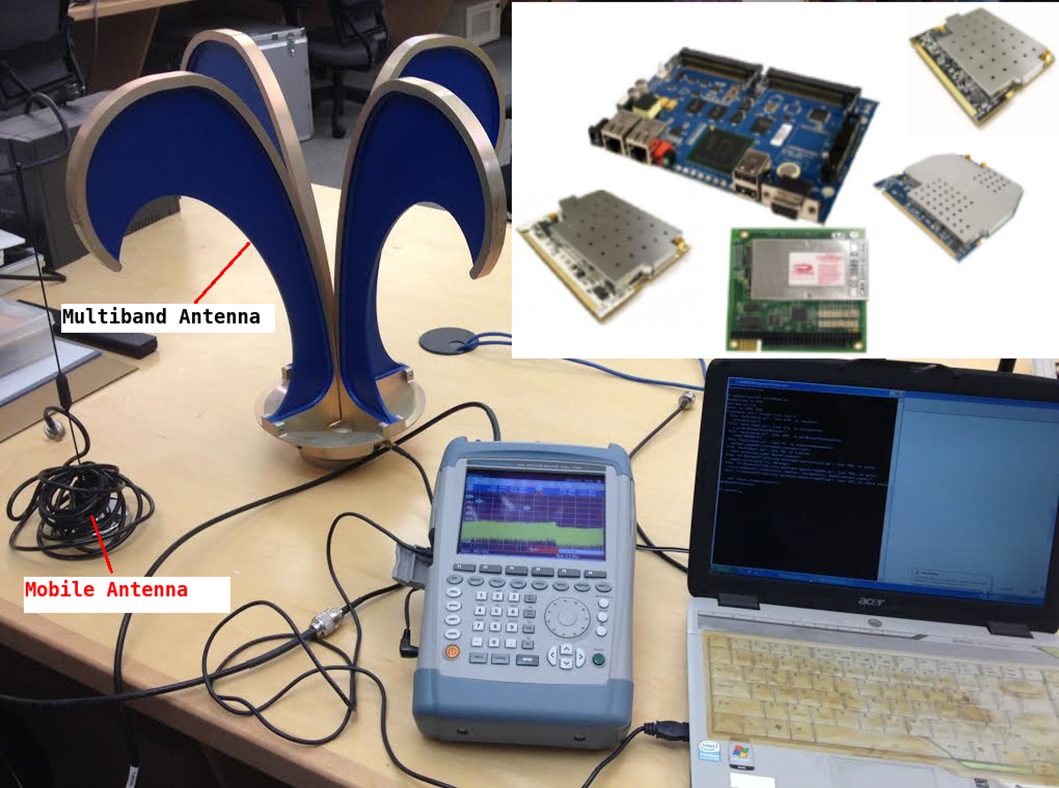
\includegraphics[width=74mm]{figures/equipment}
  \vspace{-0.1in}
  \caption{Experiment Platform}                                                                 
  \label{fig:equipment}
  %\vspace{-0.0in}
  \end{figure}
We has 64 samples each second from the spectrum analyzer system with time stamp of all bands.
Gateworks sniffer platform record all the packet received with time stamp. The duplicated 
samples are uniqued through the time stamp. Then the uniformed data are used for activity level
 calculation.  

% Location and Process 
We choose typical location according to population distribution and free white space bands from Google spectrum 
database~\cite{googledatabase}. The location chosen for experiments are marked with stars in 
Figure~\ref{dfwpopulation}.
We monitor wireless activities in each location for 2 hours in static or driving mode on a normal weekday.
Then we post-process these data to get the activities level for each band in all the location.
For our convinience, and urban areas are the most interesting in white space bands application,
we choose campus, neighborhood and bussiness area for the measurement.
 


   %\begin{figure}
   %%\vspace{-0.0in}
   %\centering
   %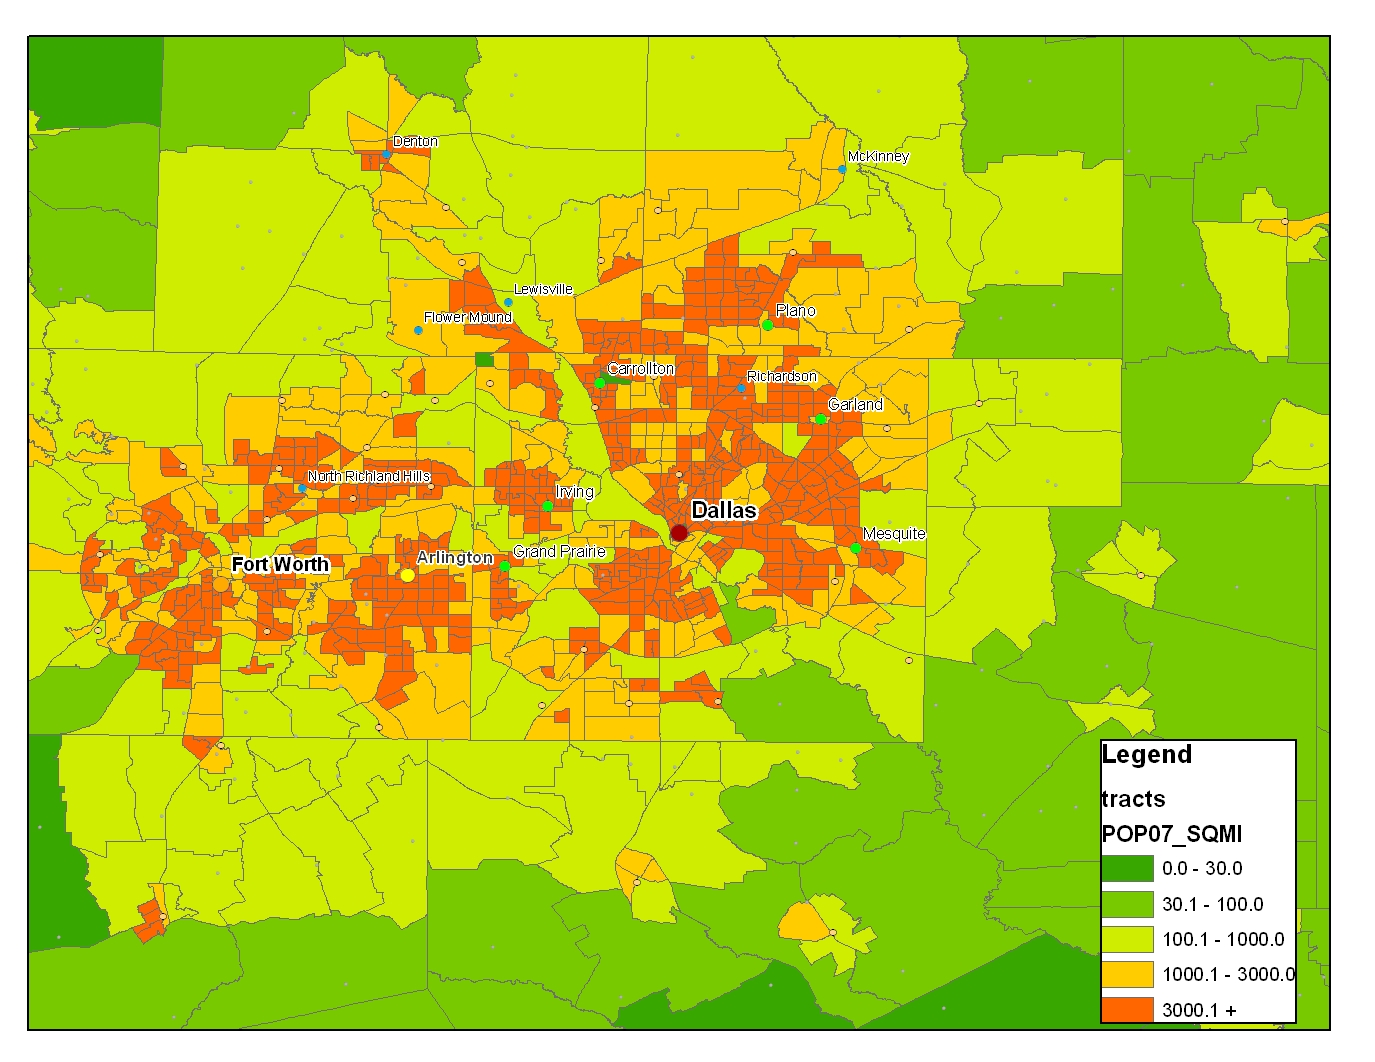
\includegraphics[width=74mm]{figures/dfwpopulation}
   %\vspace{-0.1in}
   %\caption{Dallas-Fort Worth Population Distribution}                                                                 
   %\label{fig:dfwpopulation}
   %%\vspace{-0.0in}
   %\end{figure}

% Experiment Results & expect results
In Figure~\ref{}, we show the activity level of white space bands and WiFi bands in these locations.
%White space bands activity is similar in downtown, urban area  and have a small gap from downtown to 
%rural area. That is because the long propagation of white space bands and activities are generated by 
%public TV stations most located in downtown area.
%However, the 

Based on the measured data, we apply our framework to tell the minimum access point for cover a 
certain area in different type of areas. 
We apply our framework in a x by x area in downtown, urban, urban+downtown, urban+ rural, rural
area. An access point could not occupy all the frequency spectrum, an access point could have up to
 4 radios in legal bands.
 In Figure~\ref{fixme} we show the lower bound of access point we could use to cover such an area 
 with different bands combinations.


   %\begin{figure}
   %%\vspace{-0.0in}
   %\centering
   %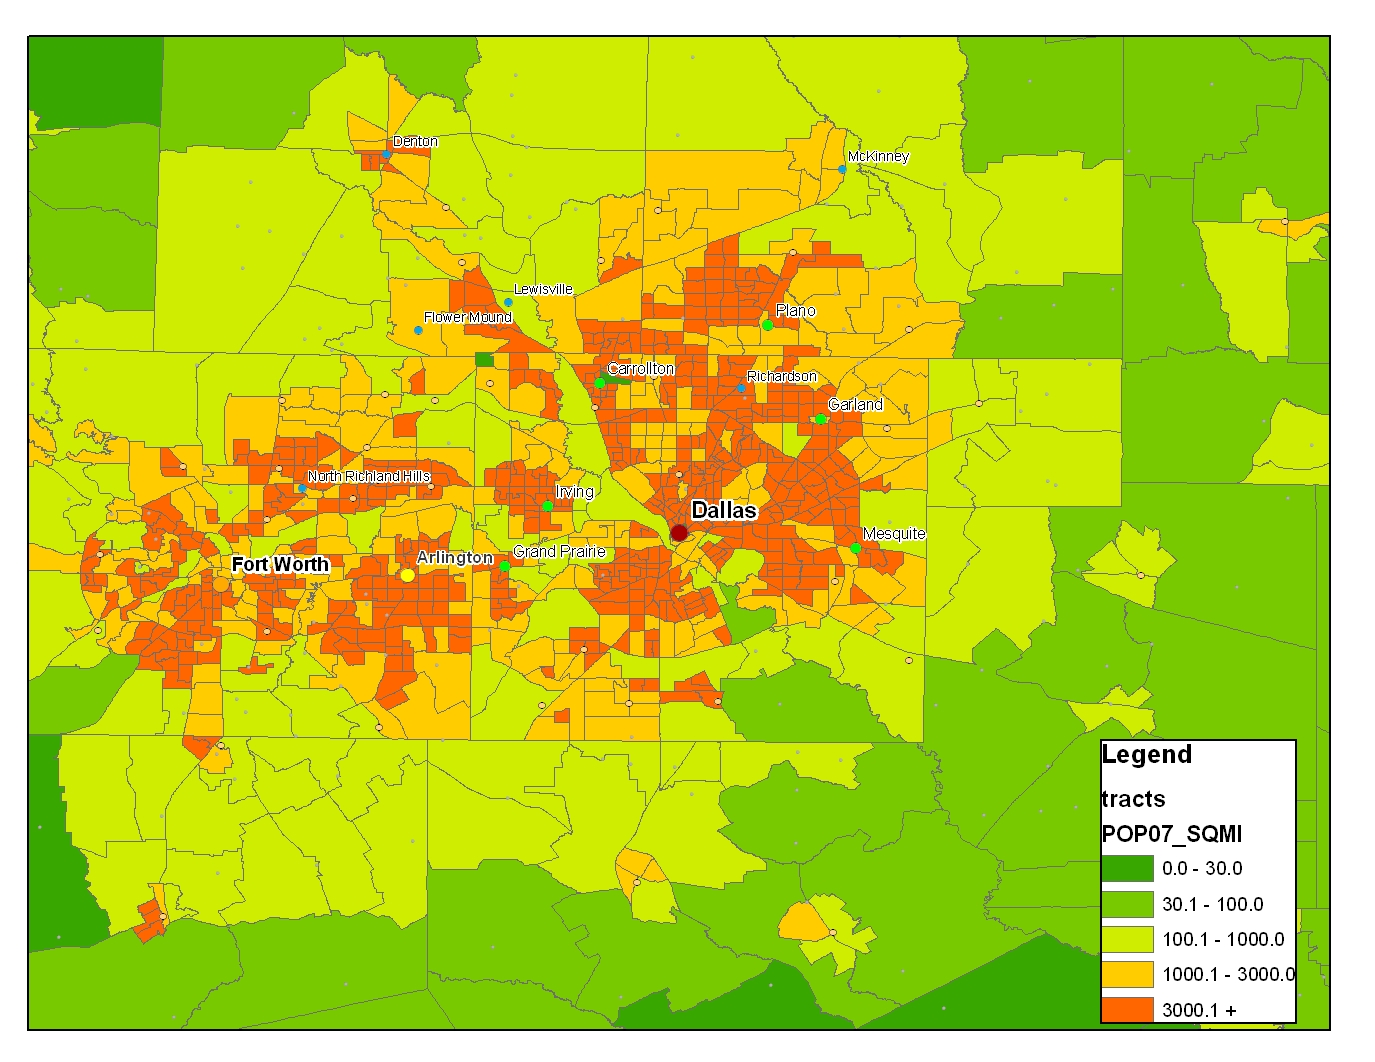
\includegraphics[width=74mm]{figures/dfwpopulation}
   %\vspace{-0.1in}
   %\caption{Dallas-Fort Worth Population Distribution}                                                                 
   %\label{fig:dfwpopulation}
   %%\vspace{-0.0in}
   %\end{figure}

In rural area, white space band is better than any other options due to the limited traffic demand;
%fixme
in downtown area
in downtown+urban area
in urban neighbor area
in urban bussiness area
in urban campus
in urban+rural area

In Figure~\ref{fixme}, when given an area mixed with urban and rural type, as urban area increase
the band selection

In Figure~\ref{fixme}, when given an area with $50\%$ rural and $50\%$ urban area, as the urban 
population density varies

In Figure~\ref{fixme}, as white space channels number increase, the access point number





